% Chapter 1

\chapter{Theoretical Introduction} % Main chapter title

\label{Chapter1} % For referencing the chapter elsewhere, use \ref{Chapter1} 

% ----------------------------------------------------------------------------------------

% Define some commands to keep the formatting separated from the content 
\newcommand{\keyword}[1]{\textbf{#1}}
\newcommand{\tabhead}[1]{\textbf{#1}}
\newcommand{\code}[1]{\texttt{#1}}
\newcommand{\file}[1]{\texttt{\bfseries#1}}
\newcommand{\option}[1]{\texttt{\itshape#1}}

% ----------------------------------------------------------------------------------------
\section{Introduction}

TODO: incluir introducción del problema.

Info:
- Handbook incluye una introducción histórica.
- Libro verde incluye una introducción intuitiva excelente.



\section{Boolean Algebra}

We could have started the topic right from the axioms. Nonetheless, given the goal we want to achieve, it seems excessive. We will refer to the commonly used \emph{Zermelo-Fraenkel axioms}, in order to have a point of reference, and therefore we will work without more considerations with sets and sets operations. We will put \emph{Zorn's lemma} to work, so the axiom of choice will also be needed, although in practice we will only work with finite sets of formulas.\\

Further on this section we will present Boolean Algebra in a classic lattice-based way that could be found in related literature. In particular we follow Introduction to mathematics of satisfiability\cite{marek2009introduction} for the definition of Booblean Algebra and Propositional Logic.

\begin{definition}
  A partial ordered set, also poset, is a pair $\{X, \le\}$ where $X$ is a set and $\le$ is a partial order of $X$. A chain $Y$ of $\{X, \le\}$ is a subset of $X$ where $\le$ is a total order. 
\end{denition}

\begin{proposition}[Zorn lemma]
  If every chain in a poset $\{X,\le\}$ is bounded, then $X$ possesses a maximal elements and for every $x\inX$ there is a maximal element $y$ such that $x\le y$.
\end{proposition}



\begin{definition} A lattice is a partial ordered set $\{X,\le\}$ where every pair of elements possesses a least upper bound and a greatest lower bound. A lattice will have two new operations defined, given two elements $x,y\in X$
  \begin{itemize}
  \item $x\vee y$ that denote the least upper bound.
  \item $x\wedge y$ that denote the greatest lower bound.
  \end{itemize}
  A lattice is complete if every subset has a unique largest element and a unique lowest element. A lattice could be presented generally as a duple $\{L,\le\}$, a triple $\{X,\vee,\wedge\}$ and, if possible, would be presented as a quintuple $\{X, \vee, \wedge, \top,\bot\}$ where $\top$ is the greatest element and $\bot$ the lowest element. a lattice is called distributive i $x\vee(y \wedge z) = (x\vee y) \wedge (x \vee z)$ and $x\wedge(y \vee z) = (x\wedge y) \vee (x \wedge z)$
\end{definition} 


With the context of lattice just included, we will present the \emph{Knaster and Tarski fixpoint theorem} fixpoint theorem. In order to do that we will introduce some notation. Given $f:\{L,\le\}\to \{L,\le\}$ a function a prefixpoint (resp. postfixpoint) is a point $x \in L$ such that $f(x) \le x$ (resp. $f(x) \ge x$). A fixpoint is a point that is both prefixpoint and postfixpoint. Note that, given that they exists, $\top$ and $bot$ are a prefixpoint and a postfixpoint of $f$ respectively.

\begin{theorem}[proposition 1.2 \cite{marek2009introduction}]
  Let $f:\{L,\le\}\to \{L,\le\}$ be a monotone function in a complete lattice. Then:
  \begin{enumerate}
  \item $f$ has a least prefixpoint $l$ that is a fixpoint.
  \item $f$ has a largest postfixpoint $l$ that is a fixpoint.
  \end{enumerate}
\end{theorem}
\begin{proof}\\
  
  \begin{enumerate}
  \item We know that there is at least a prefixpoint. Let
    $$l = \bigwedge_{\{x\in X: x\text{ is a prefixpoint}\}} x $$. 
    Lets prove that $l$ is a fixpoint. Le $x$ be an arbitrary fixpoint, therefore, $l \le x \le f(x)$. Since $x$ was arbitrary, $f(l) \le l$. To show that it a fixpoint it suffices to see that $f(l)$ is a prefixpoint to, as $f$ is monotone.
  \item Apply the previous result on $f:\{L,\le\}\to \{L,\le\}$.
  \end{enumerate}
\end{proof}

  
\begin{definition}
  A \emph{Boolean algebra} is a distributive lattice  $\{X, \vee, \wedge, \top,\bot\}$ with an additional operation $\neg$, called complement or negation, such that for all $x\inX$:
  \begin{enumerate}
  \item $ x\wedge \neg x = \bot,\ x\vee \neg x = \top $
  \item $ \neg(x \vee y) = \neg x \wedge \neg y,  \neg(x \wedge y) = \neg x \vee \neg y$
  \item $\neg \neg x = x$
  \end{enumerate}
\end{definition}
    


\section{Propositional Logic}
Propositional logic is the framework that will allow us define the main topics of this text.  Let's define some concepts:
\begin{itemize}
\item An alphabet $A$ is an arbitrary non-empty set.
\item A symbol $a$ is an element of the alphabet.
\item A word $w = \{a_i:i\in 1,..,n\}$ is a finite sequence of symbols.
\item The collection of all possible words over an alphabet $A$ is denoted by $A^*$.
\item A language $L$ over $A$ is a subset of $A^*$.
\end{itemize}

For example, Spanish is a language with a well-known alphabet. Also, Spanish is a proper language over its alphabet as it is not empty, and it does not include all possible words.\\

When we talk about a logic system we are talking about a distinguished formal language. A formal language is defined by it syntax and its semantics. The syntax is the rules that define the language. They state what words over an alphabet are valid in the language. The semantics deal with the interpretations of the elements in the language. Usually this is achieved by assigning truth values to each word.\\

We will define now propositional logic, or zeroth-order-logic. \\

\begin{figure}[h]
  \begin{center}
  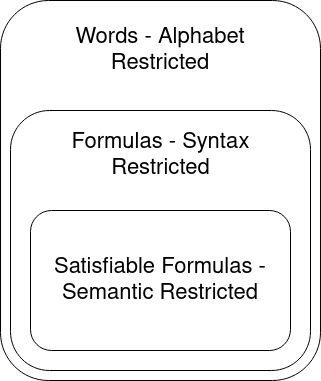
\includegraphics[width=5cm]{figures/sintax2.png}
  \caption{Diagram showing the different restrictions which may be constructed on the formal language of propositional logic.}
  \end{center}
\end{figure} 

\subsection{Syntax of Propositional Logic}
  We first start with the basic building blocks, which collectively form what is called the alphabet:
    \begin{itemize}
    \item Symbols $x,y,z$ for variables. As more variables are necessary sub-indexes will be used.
    \item Unary operator $\neg$ (negation). A literal will refer to a variable or a negated variable.
    
    \item Values 0 and 1. This values are often named as $\bot$ and $\top$ respectively.

    \item Binary operators: $\wedge, \vee, \rightarrow, \oplus, \iff $
    \end{itemize}


 The words of Propositional Logic are called formulas.
    \begin{definition}
    A Boolean formula is defined inductively:
\begin{itemize}
\item The constants 0 and 1 are formulas.
\item Every variable is a formula.
\item If $F$ is a formula, then $\neg  F$ is a formula.
\item The concatenation with a binary operator of two formulas is a formula too.\\
\end{itemize}
\end{definition}

 Examples of formulas are $x\vee y$ or $x_1\wedge x_2 \vee  ( x_4 \vee \neg  x_3 \wedge (x_5\to x_6) \vee 0 )$.We should distinguish a special type of formula: the clauses. A clause  is a formula with the form $l_1\vee ... \vee l_n$ where $l_i, i \in 1,...,n$ are literals. Clauses are will be often regarded as a finite set of literals. Example of a clause is $(x_1\vee \neg x_4 \vee x_2)$. When regarded as a set every clause $C$ has a cardinal $|C|$, that represents the number of literals contained. \\

\subsection{Semantics of Propositional Logic}
When facing a way to provide semantic meaning to formulas the use of function In this section we will discuss to ways of providing meaning to the formulas: two-valued logic and three valued logic.\\ 

    In two valued logic define the truth value of a formula by assigning a truth value(1 for Truth and 0 for False) to each variable. Note that we assign a meaning of truth to the constants 1 and 0, that until now where meaningless. The truth value of the formulas that involve operators are provide by their truth table.


\begin{table}[h]
\begin{center}
\begin{tabular}{|l|l|l|l|l|l|l|l|}
\hline
$p$ & $q$ & $\neg p$& $p\vee q$ & $p\wedge q$ & $p \oplus q$ & $p \to q $ & $p \iff q$  \\ 
\hline
  0 & 0 & 1 & 0 & 0 & 0 & 1&1\\
  0 & 1 & 1 & 1 & 0 & 1 & 1&0\\
  1 & 0 & 0 & 1 & 0 & 1 & 0&0\\
  1 & 1 & 0 & 1 & 1 & 0 & 1&1\\\hline
\end{tabular}
\end{center}
\caption{\label{tab:table-name}Truth tables of different operators in two valued logic.}
\end{table}


The truth value of a formula is therefore obtained by replacing each variable by their assigned constant and propagating the value. The tool that we will use to assign a truth value to each variable is the assignments
    \begin{definition}
      An assignment is a function $\alpha$ from the $Form_{Var}$ to $Form_{Var}$, on which some variables $\{x_1,...,x_n \}$ are replaced by predefined constants $\{a_1,...,a_n\}$ respectively.\\
    \end{definition}

    A assignment that assign a value $a$ to a variable $x$ is said to map the variable $x$. In two valued logic we will consider only assignment that maps all variables, and therefore all formulas are given a value by an assignment. We also see that any assignment generate a map from $Var$ to $\{0,1\}$. Conversely, any map from $Var$ to $\{0,1\}$ would uniquely represent a assignment $alpha$ over $Form_{Var}$. In practice when we talk about an assignment $\alpha$ we will refer indistinctly to either the function over $Form_{Var}$ or the mapping  over $Var$.\\

    One can then \emph{apply} an assignment $\alpha$ to a formula $F$, denoting it by $F\alpha=\alpha(F)$. To describe an assignment we will use a set that pairs each variable to it value, i.e. $\alpha=\{x_1\to 1,...,x_n\to 0\}$. For example given an assignment $\alpha_0 = \{x_1 \to 1, x_2\to 1, x_3 \to 0, x_4 \to 1\}$ and $F_0=x_1\to (x_2\wedge x_4)$ then  $F_0\alpha_0=1 \to (1\wedge 1)= 1$. \\    

    \begin{definition}
      An assignment is said to \emph{satisfy}  a formula $F$ if $F\alpha=1$ and in the case $F  \alpha = 0 $ it is said to \emph{falsify} the statement. A formula $F$ is called \emph{satisfiable} if is exists an assignment that satisfy it. Otherwise it is called \emph{unsatisfiable}.
    \end{definition}


    Note that we have a really restrictive constraint on the assignment: they should map all variables.  This is so in order for an assignment to give a meaning to every formula. To ease this constraint we use three-valued logic. On three valued logic we have three significant: True or 1, False or 0, and unknown or $\upsilon$. Now the assignment will map every variable to one of this values. These new assignments will be called partial assignments, as they only map some variables to a truth value. We can propagate the previous values adding new rules.

\begin{table}[h]
\begin{center}
\begin{tabular}{|l|l|l|l|l|l|l|l|}
\hline
$p$ & $q$ & $\neg p$& $p\vee q$ & $p\wedge q$ & $p \oplus q$ & $p \to q $  & $p \iff q$  \\ 
  \hline
  
  \upsilon & 0 & \upsilon & \upsilon & 0 & \upsilon & \upsilon &\upsilon\\
  \upsilon & 1 & \upsilon & 1 & \upsilon & \upsilon & 1 &\upsilon\\
  0 & \upsilon & 1 & \upsilon & 0 & \upsilon & 1 &\upsilon\\
  1 & \upsilon & 0 & 1 & \upsilon & \upsilon & \upsilon &\upsilon\\
\hline

\end{tabular}
\end{center}
\caption{\label{tab:table-name}Truth table of different operators in three valued logic.}
\end{table}


In practice partial assignments will be only define by denoting only the variables that are mapped to either 0 or 1. We can see that the composition of assignments (seen as functions over $Form_{var}$ is also a partial assignment. Also, when applying a partial assignment to a formula, instead of mapping it to $\upsilon$ we will avoid operating over the variables assigned to $\upsilon$. For example given an assignment $\alpha_0 = \{x_1 \to 1, x_2\to 1, x_3 \to 0\}$ and $F_0=x_1\to (x_2\wedge x_4)$ then  $F_0\alpha_0=1 \to (1\wedge x_4)= 1 \to (x_4)$. Although $F_0$ is mapped to another formula, $\alpha_0$ is still providing a meaning to it, i.e., that we are not sure whether this is a true or false assignment. \\



Partial assignments will be also used to iteratively expand them: let $Var= \{x_i:i\in 1,...,n\}$ the set of variables a partial assignment $\alpha_1$ that map variables $[x_1\to a_1,...,x_j\to a_j]$ with $1<j<n$ and $a_j\in\{0,1\}$ for every $j$, we can expand it by choosing a nonempty subset  $A\subset\{a_k: k\in j+1,..,n\}$ and a value $c_x \in \{0,1\}$ for every $x\in A$. Then we can define:

$$
\alpha_2(x)=
\begin{cases}
\alpha_1(x) & x \in \{x_i : i \in 1,...,n\},\\
c_x & x\in A, \\
\upsilon & \text{otherwise}.
\end{cases}
$$

We can see that $\alpha_2$ expands $\alpha_1$ in the sense that the truth value assigned to a formula by $\alpha_1$ holds in $\alpha_2$ if it where different that unknown. Therefore we are expanding the 'known' values of the formulas. Note that in the definition of $\alpha_1$ it where not necessary to state what variables were mapped to $\upsilon$ at it was implicit that every variable not listed were of unknown  value. Arguably, the most special case of partial assignment are autarks assignments[\ref{sec:autark}]. An autark assignment is an assignment that simplify a formula in a sense latter explained.\\

Two formulas $F,G$ are said to be equal, represented as $F\sim G$, if for every two-valued assignment $\alpha$ maps $F\alpha = G\alpha$. It follows from the equivalently properties on constants that $\sim$ is an equal relationship. This definition is really intuitive, as it define as equal the formulas that has the same meaning in every possible situation. \\

With $\sim$ defined we can have what is called a Lindenbaum algebra, as a quotient space of $Form = Form_{Var}$ by the relation $\sim$, denoted as $Form/\sim$. It follows that every operator respect the quotient space structure, i.e., for every $[\phi_1],[\phi_2]\in\ Form/\sim$:

\begin{itemize}
\item $\neg [\phi_1] = [\neg\phi_1]$
\item $ [\phi_1] \vee [\phi_2]= [\phi_1 \vee \phi_2]$
\item $ [\phi_1] \wedge [\phi_2]= [\phi_1 \wedge \phi_2]$
\end{itemize}

The interest of Lindenbaum algebra resides in the fact that $\{Form, \vee,\wedge,[1],[0]\}$ is a Boolean algebra, providing therefore a nexus between the algebraic formulation of the problem an its semantics.



\section{Problems}

\subsection{Decision Problems}
Computability and complexity theory attempt to answer questions regarding how to efficiently solve real-world problems. On this section we provide a formal approach to the concept of problem, and its resolution.\\

We will study the complexity of functions. In order to standardize the approach we code the input of the function and the output of the functions using words over a finite alphabet. As for every finite alphabet $A$ there is a bijective mapping from $A^*$ to $\{0,1\}^*$ we can assume when its convenient that the alphabet is $\{0,1\}$. With this convention we are now ready to define what is a decision problem.

\begin{definition}[Decision Problem\cite{arora2009computational}]
Given a language $L$ over an alphabet $A$, it has an associated decision problem that consist on, given a word $w\in A^*$ check whether $w$ is in $L$. 	
\end{definition}


When we have a named language, we refer indistinctly by this name to both the language and the associated decision problem. In order to define a decision problem is only needed to define a language over an alphabet. Therefore a decision problem may be defined implicitly, that is, as the set of the words in an alphabet that satisfy some condition. As semantics provide meaning to the languages, real world problems can be addressed as decision problems.

\subsection{Satisfiability Problem}

Given the previous definitions, we are now almost prepared to define the central part of this thesis: the satisfiability decision problem of propositional logic, SAT for short. To this end we define a special subset of formulas in Propositional Logic: the formulas in Conjunctive Normal Form.

\begin{definition}
      A formula $F$ is said to be in Conjunctive Normal Form ($CNF$)  if is written as:
      $$F = C_1\wedge ... \wedge C_n$$
      Where $C_i$  are clauses.
    \end{definition}

Note that every formula in $CNF$ can be regarded as a set of clauses. This approach is really useful in some contexts and will be often used.

\begin{definition}
  The Satisfiability Language of Propositional Logic (SAT) is the language over the alphabet of propositional logic that includes all formulas that are both satisfiable and in $CNF$.
\end{definition}

We will refer with the acronym $SAT$ to both the language and the associated decision problem. As checking if a formula is in CNF is a fairly simple syntax problem, we are only interested in asserting whether or not a formula in $CNF$ is satisfiable.

\begin{definition}
A \emph{SAT-Solver} is an algorithm that, being given a formula $F$ in \emph{CNF} as input, answer whether or not is satisfiable.
\end{definition}

We will differentiate two types of SAT-Solver. INCLUIR COMPLETOS E INCOMPLETOS.

\subsection{Variations}

The SAT decision problem quite a lot of variations, all of them of interest for certain complexity classes. We will list some of the most important, starting with two decision problems. The first of them is a natural generalization.

\begin{definition}
  The Generalized Satisfiability Language of Propositional Logic (GSAT) is the language over the alphabet of propositional logic that includes all formulas that are Satisfiable.
\end{definition}

With Tseitin's Theorem\ref{the:Tseitin} we can see that this two problems are in fact fairly similar. More often than not GSAT will be solved by solving an equivalent SAT problem. Analogously a \emph{GSAT-Solver}  is a SAT-solver that also accepts as inputs formulas not in CNF. For the next variation we will need a definition.

\begin{definition}
  Let $F$ be a formula. $F$ is said to be $k$-CNF formula (equivalently a formula in $k$-CNF) if it is in CNF and $\forall C \in F, |C| = k$. $k$-SAT is the language of the formulas that are both satisfiable and in $k$-CNF.
\end{definition}

Other variations of SAT could be achieved by generalizing the concept of decision problem.

\begin{definition}[Function Problem]
Let $A,B$ be two sets. Given a relation $R\subset A\times B$, it has an associated function problem that consists on, given a word $a\in X$ find a word $b\in B$ such that $(a,b)\in R$.
\end{definition}

That is, is the problem of finding 

\begin{definition}
 Let $Form$ be the set of propositional formulas in CNF and $B$ the set of assignments.  The Satisfiability Function Problem of Propositional Logic (FSAT) is the function problem defined by the relation $$R=\{(F, b): F\in Form, b \in B, Fb = 1\}.$$
\end{definition}
That is, is the problem of finding an assignment that satisfy a formula. Most of SAT-solvers not only try to solve SAT but also to solve FSAT, i.e., try to find an assignment that satisfy  the formula should it exists.
\begin{definition}
 Let $Form$ be the set of propositional formulas in CNF and $B$ the set of assignments. The Maximum Satisfiability Problem (MAXSAT) is the problem. function problem defined by the relation $$R=\{(F,n) : F\in Form, n = \max_{\alpha \in B}\{ | \{C\in F : C\alpha =1 \}| \}.$$
\end{definition}

That is, is the problem of finding the maximum number of assignments that can be satisfied simultaneously.


\subsection{Constraint Satisfaction Problem}

We want to introduce the notion of Constraint Satisfaction Problem (CSP) because is define a new optic over the SAT problem. 


\subsection{Autarks assignments}
\label{sec:autark}
\begin{definition}
An partial assignment $\alpha$ is called autark for a CNF formula $F$ if for every clause $C \in F$ it happens that if $Var(C) \cap Var(\alpha) \ne \emptyset $ then $C\alpha = 1$.
\end{definition}

That it satisfies all clauses that it 'touches'. The use of this definition is self-evident, as it would simplify the problem of checking whether a CNF formula $F$ is satisfiable. When we apply an autark assignment to $F$ we generate another formula $F\alpha \subset F$\\.

These assignments provide simplifications of the CNF Formulas in the context of satisfiablity,

    Should it happen that we got an algorithm for autarks clauses, and iterating it, we could find a solution of any given formula. Finding a polynomial algorithm that finds whether there exists any non-empty autark formula and provide it, we could be able of proving that NP = P, as we could solve SAT applying this algorithm iteratively. Anyway, trying to find simple autark assignment, i.e. assignment with not many variables,is a good praxis.

    \begin{proposition} We could reduce SAT to the Autark-Finding problem.
      \begin{proof} Suppose that an algorithm such that if it exists any autark it return one of them, and end with an error code otherwise is given.  \\

        Given a formula $F$, if there is not an autark then there is no solution for the SAT problem. If it finds an Autark-assignment $\alpha$ then we apply the same algorithm to $\alpha(F)$. Also, as it happens that $|Var(\alpha(F))|<|Var(F)|$ so we would only apply the algorithm finitely many times. Also, $F$ will be solvable if, and only if, $F\alpha$ is solvable.	\\

        Moreover, as checking whether an assignment is autark is linear on the number of clauses, then this make the autark-finding problem NP-Complete(NP-C further on).
      \end{proof}
      
    \end{proposition}



\section{Models of Computation}
On this section we will discuss two computation models: Turing Machines and Circuits. We do not expect the text to be the first approximations to Turing machines, so we present a quick formal approach to the area. 

\subsection{Turing Machines}
Turing machines are arguably the epicenter of  models of computation. A Turing Machine  represents a long mechanical tape on which we are going to operate. The tape is divided in to discrete positions, such that we can see the tape as a one-dimensional array. Operating on this tape we can focus on a cell, scan its contents, overwrite  its contents or move to an adjacent cell. These operations try to resemble the process of human calculus, as done with paper and pencil when applying the long division method  for example. Formally:

\begin{definition}[Turing Machine \cite{hopcroft2007introduction}] We describe a Turing Machine as a 7-tuple $M=(Q, \sum, \Gamma, \delta, q_0, B, F)$ whose components have the following meanings:
  \begin{itemize}
  \item $Q$ the finite set of \emph{states} of the finite control.
  \item $\sum$ the finite set of \emph{input symbols}.
  \item $\Gamma$ the finite set of \emph{tape symbols}. $\sum$ is always a subset of $\Gamma$.
  \item  $\delta: Q\times \Gamma \to Q\times\Gamma\times\{L,R\}$ the transition function.
  \item $q_0$ the \emph{start state}.
  \item $B$ the \emph{blank symbol}.
  \item $F$ the \emph{accepting states}.
  \end{itemize}

  A configuration of a Turing machine is a triplet $C=(q,u,v)$ where $q\in Q$, $u,v\in \Gamma^*$. A configuration is accepting if $q\in F$.
\end{definition}

A configuration should be understand as a state of the machine, where $q$ is the current state, $u$ the part of the tape left to the cell on which we focus and $v$ is the part of the tape right to the cell we focus, starting on it.\\

We can define a relation between configurations that will allow us to formalize the operations that can be made on a Turing machine.

\begin{definition}
  Let $M$ be a Turing Machine and $C = (q,u_1...u_n, av_1....v_m)$, $C'=(q',u_1...u_{n-1},)$ be a configuration. We say that $C\vdash C'$ if:
  \begin{itemize}
    \item It exists $\delta(q,a) = (q',b,I)$, 
\end{definition}


\begin{enumerate}
\item PASO DE CALCULO
\item ACEPTAR RECHAZAR
\item COMPLEJIDAD ALGORITMICA
\end{enumerate}
  


\subsection{First order Logic}

\subsection{Modal Logic}




    \begin{definition}
 The set of all satisfiable formulas is denoted as $SAT$.  The problem $SAT$ is the associated problem. 	An assignment $\alpha$ that satisfies $F$ is called a model an is denoted as $\alpha \models F$.\end{definition}
    A formula $F$ such that for every  $\alpha$ assignment happens that $F\alpha=1$ is a tautology. Given two formulas $G,F$ it is said that $G$ follows from $F$ if $F\to G$ is a tautology. \\
   
    \end{definition}
      If none of the variables altered by an assignment $\alpha$ are present on the formula $F$ then $\alpha(F) = F$. We denote as $Var(\alpha)$ the set of those variables that receive a value from $\alpha$. Analogously, $Var(F)$ will denote the variables present on a formula $F$.

    
      A formula in \emph{CNF} could be seen as a collection of clauses. The associated problem with \emph{CNF} is straightforward on $O(n)$. The problem that we will investigate is whether a arbitrary formula $F$ have a \emph{SAT-equivalent} \emph{CNF} formula.\\
      
    Equivalently a clause could be seen as a set of literals. The set of all formulas in conjunctive normal form where $|C_i| = N\ i \in 1,...,n$ is called \emph{NCNF}. The intersection of these set with the \emph{SAT} sets are called \emph{CNF-SAT} y \emph{NCNF-SAT}. If the context is clear enough the problems will be called \emph{CNF} and \emph{NCNF}\\


    TODO: Definir un circuito.
    
    \begin{lemma}
      For every \emph{SAT} formula there is an associated circuit.
    \end{lemma}
    \begin{proof}
      Every operator can be seen as a gate and every variable as an input.\\
    \end{proof}
    
    \begin{theorem}[Tseitin \cite{tseitin1983complexity}] \label{the:Tseitin}
      There is a \emph{3-CNF} formula on each equivalent class. Moreover, given an element $F$  there is a equivalent formula $G$  in \emph{3-CNF} which could be computed in polynomial time. 
    \end{theorem}

    \begin{proof}
      We will show that for every circuit with $n$ inputs and $m$ binary gates there is a formula in \emph{3-CNF}  that could be constructed in polynomial time in $n$ and $m$. Then, given a formula we will work with it considering its associated circuit.\\
<
      We will construct the formula considering variables $x_1,...,x_n$ that will represent the inputs and $y_1,...,y_m$ that will represents the output of each gate. 

      $$ G = (y_1) \wedge \bigwedge_{i=1}^m (y_i \iff f_i(z_{i,1},z_{i,2}))$$

      Where $f_i$ represents the formula associated to the $i$-gate, $z_{i,1},z_{i,2}$ each of the two inputs of the $i$-gate, whether they are $x_-$ or $y_-$ variables. This formula is not \emph{3-CNF} yet, but for each configuration being $f_i$ a Boolean operator there would be a \emph{3-CNF} equivalent.

      \begin{itemize}
      \item $z \iff( x \vee y )  = \neg  ( z \vee  x \vee y    ) \vee (z \wedge ( x \vee y )  ) = \neg  ( z \vee  x \vee y    ) \vee (z \wedge x)  \vee (z \wedge y ) =$\\$= ( \neg  z \wedge  \neg  x \wedge \neg   y    ) \vee (z \wedge x)  \vee (z \wedge y )  =$$
        (\neg  z \vee (z \wedge x)  \vee (z \wedge y ))  \wedge  
        (\neg  x \vee (z \wedge x)  \vee (z \wedge y )) \wedge
        (\neg  y \vee (z \wedge x)  \vee (z \wedge y ))   =
        (\neg  z \vee x  \vee y )  \wedge  
        (\neg  x \vee z  ) \wedge
        (\neg  y \vee z ) $   
      \item $z \iff( x \wedge y ) = \neg ( z \vee ( x \wedge y )) \vee (z \wedge ( x \wedge y )) = (z\wedge x \wedge y ) \vee  (\neg  z\wedge \neg  x \wedge \neg  y )  =$\\$\ \ \ ((z\vee  (\neg  z\wedge \neg  x \wedge \neg  y )  ) \wedge (x \vee  (\neg  z\wedge \neg  x \wedge \neg  y )  ) \wedge (y\vee  (\neg  z\wedge \neg  x \wedge \neg  y )  ) ) = (\neg  x \vee z) \wedge (\neg  y \vee z ) \wedge (\neg  z \vee x ) \wedge (\neg  y \vee x ) \wedge(\neg  z\vee y )\wedge (\neg  x\vee y )$
	
      \item $z \iff( x \iff y ) =  \neg ( z \vee ( x \iff y ) ) \vee (z \wedge ( x \iff y ) = \neg ( z \vee (\neg  x \wedge \neg  y) \vee (x \wedge y)) \vee (z \wedge(\neg  x \wedge \neg  y) \vee (x \wedge y))  )=(\neg  z \wedge \neg  (\neg  x \wedge \neg  y) \wedge \neg  (x \wedge y)) \vee (z \wedge(\neg  x \wedge \neg  y) \vee (x \wedge y))  )=(\neg  z \wedge  (x \vee  y) \wedge (\neg  x \vee \neg  y)) \vee (z \wedge(\neg  x \wedge \neg  y) \vee (x \wedge y))  )=z \vee ( \neg  x \wedge \neg  y) = (\neg x \vee \neg y \vee z) \wedge (\neg x \vee \neg z \vee y) \wedge (y \vee z \vee x) \wedge (y \vee \neg y \vee x) \wedge (\neg z \vee z \vee x) \wedge (\neg z \vee \neg y \vee x)$
	
      \item $z \iff( x \oplus y ) =  z \iff(\neg  x \iff y )  $	

      \end{itemize}
      In the last item we use the third one.
      
    \end{proof}
    This result is important because, now we could be able to talk only about \emph{3-CNF} formulas. The fact that they are reachable on polynomial time is important because it means it could be done efficiently. Should this be impossible it will not be of much relevance in practice, as we yearn to solve this problem as efficient as possible (in fact, as polynomial as possible). This result implies that if we know how to solve \emph{3-CNF} then we will be able to solve 'full'SAT problems.
    \begin{definition}


    \begin{proposition}
      Given a tautology $F \to G$, there exists a formula $I$ such that $Var(I) = Var(F)\cap Var(G)$ and both $F\to I$ and $I \to G$ are tautologies. A polynomial algorithm to solve this problem is not known. 
    \end{proposition}

    \begin{proof} Let $\{x_1,...,x_k\} = Var(F)\cup Var(G)$ then we will build $I$ by defining its truth table in the following way: Given an assignment $\alpha$:
      \[   
        I\alpha = 
        \begin{cases}
          1&\quad\text{if $\alpha$ could be extended to an assignment that \emph{satisfies} $F$}, \\
          0&\quad\text{if $\alpha$ could be extended to an assignment that \emph{nullifies} $G$},\\
          * &\quad\text{otherwise.} \\ 
        \end{cases}
      \]

      Where * mean that it could be either 0 or 1.  This is well defined because if for an arbitrary $\alpha$ it happens that $G\alpha = 0$ then $F\alpha = 0$.

      For every assignment $\beta$ such that $Var(\beta) = Var(F)\cup Var(G)$ then if $\beta(F) = 1$ then $\beta(I) = 1$ so $F \to I$  is a tautology. Similarly it can not happen that $I\beta = 1 $ and $G\beta = 0$, because the second will imply that   $I\beta = 0$.\\

      For the last part we will refer to the paper on the topic by: \red{TODO}



    \end{proof}

